% Graphic for TeX using PGF
% Title: /home/lauri/msc-thesis/dia/pooled-partitioning.dia
% Creator: Dia v0.97.3
% CreationDate: Sun Apr  5 10:00:44 2015
% For: lauri
% \usepackage{tikz}
% The following commands are not supported in PSTricks at present
% We define them conditionally, so when they are implemented,
% this pgf file will use them.
\ifx\du\undefined
  \newlength{\du}
\fi
\setlength{\du}{15\unitlength}
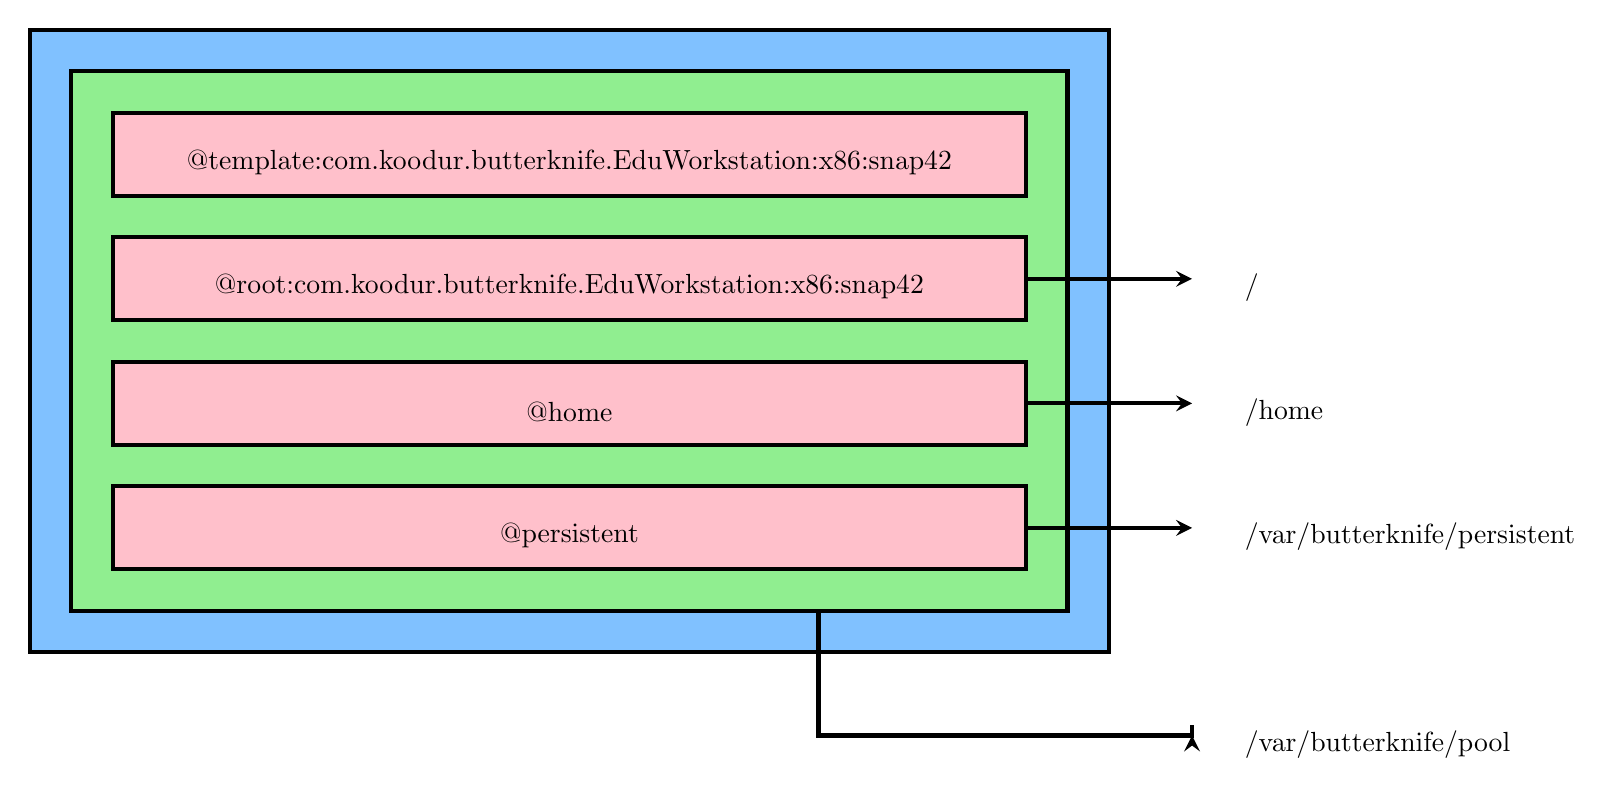
\begin{tikzpicture}
\pgftransformxscale{1.000000}
\pgftransformyscale{-1.000000}
\definecolor{dialinecolor}{rgb}{0.000000, 0.000000, 0.000000}
\pgfsetstrokecolor{dialinecolor}
\definecolor{dialinecolor}{rgb}{1.000000, 1.000000, 1.000000}
\pgfsetfillcolor{dialinecolor}
\pgfsetlinewidth{0.100000\du}
\pgfsetdash{}{0pt}
\pgfsetdash{}{0pt}
\pgfsetmiterjoin
\definecolor{dialinecolor}{rgb}{0.501961, 0.756863, 1.000000}
\pgfsetfillcolor{dialinecolor}
\fill (0.000000\du,0.000000\du)--(0.000000\du,15.000000\du)--(26.000000\du,15.000000\du)--(26.000000\du,0.000000\du)--cycle;
\definecolor{dialinecolor}{rgb}{0.000000, 0.000000, 0.000000}
\pgfsetstrokecolor{dialinecolor}
\draw (0.000000\du,0.000000\du)--(0.000000\du,15.000000\du)--(26.000000\du,15.000000\du)--(26.000000\du,0.000000\du)--cycle;
\definecolor{dialinecolor}{rgb}{0.564706, 0.933333, 0.564706}
\pgfsetfillcolor{dialinecolor}
\fill (1.000000\du,1.000000\du)--(1.000000\du,14.000000\du)--(25.000000\du,14.000000\du)--(25.000000\du,1.000000\du)--cycle;
\pgfsetlinewidth{0.100000\du}
\pgfsetdash{}{0pt}
\pgfsetdash{}{0pt}
\pgfsetmiterjoin
\definecolor{dialinecolor}{rgb}{0.000000, 0.000000, 0.000000}
\pgfsetstrokecolor{dialinecolor}
\draw (1.000000\du,1.000000\du)--(1.000000\du,14.000000\du)--(25.000000\du,14.000000\du)--(25.000000\du,1.000000\du)--cycle;
% setfont left to latex
\definecolor{dialinecolor}{rgb}{0.000000, 0.000000, 0.000000}
\pgfsetstrokecolor{dialinecolor}
\node at (13.000000\du,7.695000\du){};
\definecolor{dialinecolor}{rgb}{1.000000, 0.752941, 0.796078}
\pgfsetfillcolor{dialinecolor}
\fill (2.000000\du,2.000000\du)--(2.000000\du,4.000000\du)--(24.000000\du,4.000000\du)--(24.000000\du,2.000000\du)--cycle;
\pgfsetlinewidth{0.100000\du}
\pgfsetdash{}{0pt}
\pgfsetdash{}{0pt}
\pgfsetmiterjoin
\definecolor{dialinecolor}{rgb}{0.000000, 0.000000, 0.000000}
\pgfsetstrokecolor{dialinecolor}
\draw (2.000000\du,2.000000\du)--(2.000000\du,4.000000\du)--(24.000000\du,4.000000\du)--(24.000000\du,2.000000\du)--cycle;
% setfont left to latex
\definecolor{dialinecolor}{rgb}{0.000000, 0.000000, 0.000000}
\pgfsetstrokecolor{dialinecolor}
\node at (13.000000\du,3.195000\du){@template:com.koodur.butterknife.EduWorkstation:x86:snap42};
\definecolor{dialinecolor}{rgb}{1.000000, 0.752941, 0.796078}
\pgfsetfillcolor{dialinecolor}
\fill (2.000000\du,5.000000\du)--(2.000000\du,7.000000\du)--(24.000000\du,7.000000\du)--(24.000000\du,5.000000\du)--cycle;
\pgfsetlinewidth{0.100000\du}
\pgfsetdash{}{0pt}
\pgfsetdash{}{0pt}
\pgfsetmiterjoin
\definecolor{dialinecolor}{rgb}{0.000000, 0.000000, 0.000000}
\pgfsetstrokecolor{dialinecolor}
\draw (2.000000\du,5.000000\du)--(2.000000\du,7.000000\du)--(24.000000\du,7.000000\du)--(24.000000\du,5.000000\du)--cycle;
% setfont left to latex
\definecolor{dialinecolor}{rgb}{0.000000, 0.000000, 0.000000}
\pgfsetstrokecolor{dialinecolor}
\node at (13.000000\du,6.195000\du){@root:com.koodur.butterknife.EduWorkstation:x86:snap42};
\definecolor{dialinecolor}{rgb}{1.000000, 0.752941, 0.796078}
\pgfsetfillcolor{dialinecolor}
\fill (2.000000\du,8.000000\du)--(2.000000\du,10.000000\du)--(24.000000\du,10.000000\du)--(24.000000\du,8.000000\du)--cycle;
\pgfsetlinewidth{0.100000\du}
\pgfsetdash{}{0pt}
\pgfsetdash{}{0pt}
\pgfsetmiterjoin
\definecolor{dialinecolor}{rgb}{0.000000, 0.000000, 0.000000}
\pgfsetstrokecolor{dialinecolor}
\draw (2.000000\du,8.000000\du)--(2.000000\du,10.000000\du)--(24.000000\du,10.000000\du)--(24.000000\du,8.000000\du)--cycle;
% setfont left to latex
\definecolor{dialinecolor}{rgb}{0.000000, 0.000000, 0.000000}
\pgfsetstrokecolor{dialinecolor}
\node at (13.000000\du,9.195000\du){@home};
\definecolor{dialinecolor}{rgb}{1.000000, 0.752941, 0.796078}
\pgfsetfillcolor{dialinecolor}
\fill (2.000000\du,11.000000\du)--(2.000000\du,13.000000\du)--(24.000000\du,13.000000\du)--(24.000000\du,11.000000\du)--cycle;
\pgfsetlinewidth{0.100000\du}
\pgfsetdash{}{0pt}
\pgfsetdash{}{0pt}
\pgfsetmiterjoin
\definecolor{dialinecolor}{rgb}{0.000000, 0.000000, 0.000000}
\pgfsetstrokecolor{dialinecolor}
\draw (2.000000\du,11.000000\du)--(2.000000\du,13.000000\du)--(24.000000\du,13.000000\du)--(24.000000\du,11.000000\du)--cycle;
% setfont left to latex
\definecolor{dialinecolor}{rgb}{0.000000, 0.000000, 0.000000}
\pgfsetstrokecolor{dialinecolor}
\node at (13.000000\du,12.195000\du){@persistent};
\pgfsetlinewidth{0.100000\du}
\pgfsetdash{}{0pt}
\pgfsetdash{}{0pt}
\pgfsetbuttcap
{
\definecolor{dialinecolor}{rgb}{0.000000, 0.000000, 0.000000}
\pgfsetfillcolor{dialinecolor}
% was here!!!
\pgfsetarrowsend{stealth}
\definecolor{dialinecolor}{rgb}{0.000000, 0.000000, 0.000000}
\pgfsetstrokecolor{dialinecolor}
\draw (24.000000\du,6.000000\du)--(28.000000\du,6.000000\du);
}
\pgfsetlinewidth{0.100000\du}
\pgfsetdash{}{0pt}
\pgfsetdash{}{0pt}
\pgfsetbuttcap
{
\definecolor{dialinecolor}{rgb}{0.000000, 0.000000, 0.000000}
\pgfsetfillcolor{dialinecolor}
% was here!!!
\pgfsetarrowsend{stealth}
\definecolor{dialinecolor}{rgb}{0.000000, 0.000000, 0.000000}
\pgfsetstrokecolor{dialinecolor}
\draw (24.000000\du,9.000000\du)--(28.000000\du,9.000000\du);
}
\pgfsetlinewidth{0.100000\du}
\pgfsetdash{}{0pt}
\pgfsetdash{}{0pt}
\pgfsetbuttcap
{
\definecolor{dialinecolor}{rgb}{0.000000, 0.000000, 0.000000}
\pgfsetfillcolor{dialinecolor}
% was here!!!
\pgfsetarrowsend{stealth}
\definecolor{dialinecolor}{rgb}{0.000000, 0.000000, 0.000000}
\pgfsetstrokecolor{dialinecolor}
\draw (24.000000\du,12.000000\du)--(28.000000\du,12.000000\du);
}
% setfont left to latex
\definecolor{dialinecolor}{rgb}{0.000000, 0.000000, 0.000000}
\pgfsetstrokecolor{dialinecolor}
\node[anchor=west] at (29.000000\du,9.221250\du){/home};
% setfont left to latex
\definecolor{dialinecolor}{rgb}{0.000000, 0.000000, 0.000000}
\pgfsetstrokecolor{dialinecolor}
\node[anchor=west] at (29.000000\du,12.221250\du){/var/butterknife/persistent};
% setfont left to latex
\definecolor{dialinecolor}{rgb}{0.000000, 0.000000, 0.000000}
\pgfsetstrokecolor{dialinecolor}
\node[anchor=west] at (29.000000\du,6.221250\du){/};
% setfont left to latex
\definecolor{dialinecolor}{rgb}{0.000000, 0.000000, 0.000000}
\pgfsetstrokecolor{dialinecolor}
\node[anchor=west] at (29.000000\du,17.221250\du){/var/butterknife/pool};
\pgfsetlinewidth{0.100000\du}
\pgfsetdash{}{0pt}
\pgfsetdash{}{0pt}
\pgfsetmiterjoin
\pgfsetbuttcap
{
\definecolor{dialinecolor}{rgb}{0.000000, 0.000000, 0.000000}
\pgfsetfillcolor{dialinecolor}
% was here!!!
\pgfsetarrowsend{stealth}
{\pgfsetcornersarced{\pgfpoint{0.000000\du}{0.000000\du}}\definecolor{dialinecolor}{rgb}{0.000000, 0.000000, 0.000000}
\pgfsetstrokecolor{dialinecolor}
\draw (19.000000\du,14.000000\du)--(19.000000\du,17.000000\du)--(28.000000\du,17.000000\du)--(28.000000\du,17.000000\du);
}}
\end{tikzpicture}
